\paragraph{Sơ đồ tuần tự luồng tra cứu lịch sử giao dịch}

Luồng nghiệp vụ này mô tả
quy trình User tra cứu danh sách giao dịch thanh toán mua gói thuê bao VIP. Web Frontend gọi dịch vụ thanh toán qua API Gateway, backend truy vấn transaction.

\begin{figure}[H]
\centering
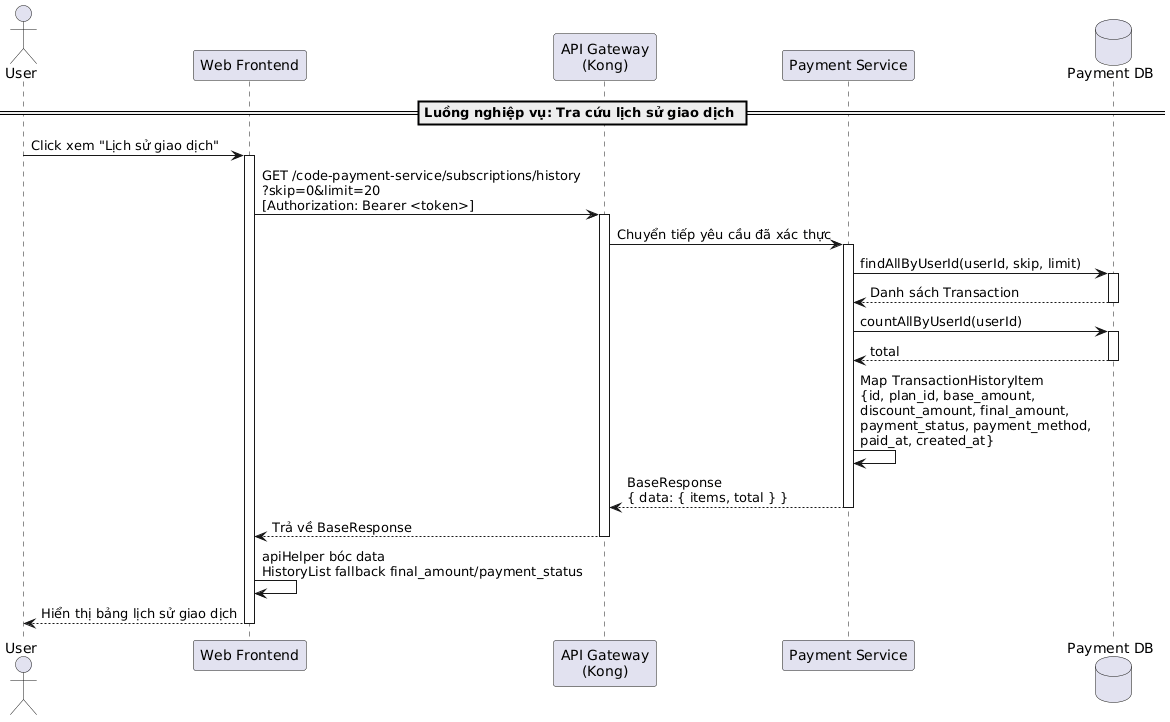
\includegraphics[width=0.95\textwidth]{contents/Sequence/UML-Sequence-UserTransactionHistoryLookup.png}
\caption{Sơ đồ tuần tự luồng tra cứu lịch sử giao dịch}
\end{figure}

\subparagraph{Mô tả tổng quan}

\begin{itemize}

\item \textbf{Yêu cầu xem lịch sử:}
Người dùng mở trang lịch sử giao dịch.
Giao diện gửi yêu cầu lấy danh sách lịch sử qua cổng API kèm theo các tham số phân trang.

\item \textbf{Truy vấn lịch sử giao dịch:}
Dịch vụ thanh toán
tiếp nhận yêu cầu, truy vấn CSDL để lấy danh sách các giao dịch thanh toán và tổng số lượng giao dịch của người dùng.

\item \textbf{Chuyển đổi dữ liệu:}
Dịch vụ thanh toán
chuyển đổi danh sách các giao dịch sang cấu trúc dữ liệu hiển thị.

\item \textbf{Hiển thị kết quả:}
Dịch vụ thanh toán
phản hồi danh sách giao dịch cùng tổng số lượng về giao diện.
Giao diện tiếp nhận dữ liệu
và hiển thị chi tiết số tiền thanh toán thực tế cùng trạng thái của từng giao dịch lên màn hình lịch sử.
\end{itemize}

\begin{table}[H]
\centering
\renewcommand{\arraystretch}{1.3}

\begin{tabular}{|l|l|p{5cm}|}
\hline
\textbf{Thành phần} & \textbf{Phân loại} & \textbf{Vai trò trong hệ thống} \\ \hline
User & Actor & Người dùng yêu cầu tra cứu lịch sử giao dịch cá nhân. \\ \hline
Web Frontend & Component & Giao diện web Next.js. \\ \hline
API Gateway (Kong) & Component & Cổng API chuyển tiếp các yêu cầu API. \\ \hline
Payment Service & Microservice & Tiếp nhận query, lấy danh sách transaction và tổng số bản ghi theo \texttt{userId}. \\ \hline
Payment DB & Database & Lưu thông tin Transaction của người dùng. \\ \hline
\end{tabular}
\caption{Các thành phần tham gia luồng tra cứu lịch sử giao dịch}
\end{table}
